% ==============================================================================
% results_evaluation.tex -- Section VII: Results, Evaluation, and Failure Analysis
% Author: Team Member 4 (Evaluation, Error Analysis & Visualization Lead)
% ==============================================================================

\section{Experimental Results and Evaluation}
\label{sec:results_evaluation}

This section provides a rigorous, standardized evaluation across all localization models developed throughout the project. 
To guarantee methodological integrity and prevent data snooping, all classical baselines, single-task deep networks, multitask deep architectures, and hybrid systems are evaluated on the exact same held-out benchmark test set ($N = 1{,}111$ scans from the official \texttt{validationData.csv} of the UJIIndoorLoc corpus).

\subsection{Standardized Evaluation Metrics}

Indoor positioning requires simultaneous assessment of hierarchical discrete identification (building and floor) and continuous spatial regression (coordinates):
\begin{enumerate}
    \item \textbf{Building and Floor Accuracy:} Classification accuracy, macro-averaged precision, recall, and $F_1$-score:
    \begin{equation}
        \text{Acc} = \frac{1}{N} \sum_{i=1}^N \mathbb{I}(\hat{y}_i = y_i), \quad F_{1,\text{macro}} = \frac{1}{|\mathcal{C}|} \sum_{c \in \mathcal{C}} \frac{2 P_c R_c}{P_c + R_c}.
    \end{equation}
    \item \textbf{Joint Building--Floor Accuracy:} A prediction is considered correct if and only if \emph{both} building and floor match the ground truth simultaneously:
    \begin{equation}
        \text{Acc}_{\text{joint}} = \frac{1}{N} \sum_{i=1}^N \mathbb{I}(\hat{b}_i = b_i \;\land\; \hat{f}_i = f_i).
    \end{equation}
    \item \textbf{2D Euclidean Positioning Error:} Spatial error $d_i$ (metres) between true coordinates $(x_i, y_i)$ and predicted coordinates $(\hat{x}_i, \hat{y}_i)$ defined in the metric Universal Transverse Mercator (UTM) coordinate system:
    \begin{equation}
        d_i = \sqrt{(x_i - \hat{x}_i)^2 + (y_i - \hat{y}_i)^2}.
    \end{equation}
    We report the mean, median (50th percentile), 75th percentile ($P_{75}$), 90th percentile ($P_{90}$), and maximum error. Coordinate MAE, RMSE, and coefficient of determination ($R^2$) are also computed.
    \item \textbf{EvAAL Competition Score:} The internationally recognized Evaluating Ambient Assisted Living (EvAAL) benchmark score incorporates domain-specific penalty terms for hierarchical boundary violations:
    \begin{equation}
        \mathcal{S}_{\text{EvAAL}} = \frac{1}{N} \sum_{i=1}^N \left[ d_i + 50 \cdot \mathbb{I}(\hat{b}_i \neq b_i) + 4 \cdot |f_i - \hat{f}_i| \right].
    \end{equation}
\end{enumerate}

% ------------------------------------------------------------------------------
% Table: Master Benchmark Comparison
% ------------------------------------------------------------------------------
\begin{table*}[t]
\centering
\caption{Comprehensive Benchmark Model Comparison on the Held-out Test Set ($N = 1{,}111$)}
\label{tab:final_comparison}
\renewcommand{\arraystretch}{1.2}
\setlength{\tabcolsep}{5pt}
\begin{tabular}{@{}llccccccccc@{}}
\toprule
\textbf{Model Architecture} & \textbf{Paradigm} & \textbf{Bldg Acc} & \textbf{Floor Acc} & \textbf{Joint Acc} & \textbf{Mean Err} & \textbf{Med Err} & $\mathbf{P_{75}\text{ Err}}$ & $\mathbf{P_{90}\text{ Err}}$ & $\mathbf{R^2}$ & \textbf{EvAAL} \\
 & & \textbf{(\%)} & \textbf{(\%)} & \textbf{(\%)} & \textbf{(m)} & \textbf{(m)} & \textbf{(m)} & \textbf{(m)} & & \textbf{Score} \\
\midrule
Random Forest (Phase 1 Baseline)      & Classical ML & 99.73\% & 89.92\% & 89.74\% & 12.30 & 8.15 & 15.65 & 29.55 & 0.978 & 13.04 \\
Extra Trees Regressor                 & Classical ML & 99.73\% & 89.92\% & 89.74\% & 12.46 & 7.66 & 15.42 & 25.68 & 0.971 & 13.20 \\
$k$-NN ($k=5$, distance-weighted)     & Classical ML & 98.92\% & 75.43\% & 75.16\% & 13.68 & 8.20 & 15.75 & 29.21 & 0.964 & 15.54 \\
XGBoost                               & Classical ML & 99.82\% & 89.56\% & 89.56\% & 22.70 & 15.17 & 29.80 & 47.77 & 0.940 & 23.41 \\
\midrule
Single-Task Deep Networks             & Deep Learning & \textbf{100.00\%} & 91.90\% & 91.90\% & 8.66 & 6.37 & 10.95 & \textbf{17.13} & 0.984 & 9.02 \\
Multitask Neural Network (Phase 2)    & Deep Learning & 99.73\% & 91.00\% & 91.00\% & 8.95 & 7.04 & 11.05 & 17.87 & 0.982 & 9.50 \\
Hybrid Stacking (DL + Tree Probs)     & Hybrid DL+ML & 99.82\% & \textbf{92.08\%} & \textbf{92.08\%} & 8.86 & 6.69 & 11.04 & 17.72 & 0.983 & 9.31 \\
Hybrid Residual Correction (DL + GBDT)& Hybrid DL+ML & 99.73\% & 91.00\% & 91.00\% & 8.75 & 6.69 & 11.07 & 17.59 & 0.983 & 9.29 \\
\textbf{Full Hybrid (Stacked DL + GBDT)} & \textbf{Hybrid DL+ML} & 99.82\% & \textbf{92.08\%} & \textbf{92.08\%} & \textbf{8.51} & \textbf{6.30} & \textbf{10.72} & 17.58 & \textbf{0.984} & \textbf{8.96} \\
\bottomrule
\end{tabular}
\end{table*}

\subsection{Cross-Model Performance Synthesis}

The experimental results across all nine architectures are summarized in Table~\ref{tab:final_comparison}. Key empirical insights emerge:
\begin{enumerate}
    \item \textbf{Deep Learning vs.\ Classical Trees:} Transitioning from the best classical model (Random Forest) to the Multitask Neural Network reduces the mean positioning error from $12.30$\,m to $8.95$\,m (a $27.2\%$ error reduction), while improving the median error from $8.15$\,m to $7.04$\,m and floor accuracy from $89.92\%$ to $91.00\%$. This demonstrates that the deep continuous latent manifold learned by the shared trunk overcomes the piecewise-constant step-function limitation inherent to decision tree regression.
    \item \textbf{Synergy of Hybrid Architectures:} The Full Hybrid model (combining tree probability stacking with residual gradient boosting) achieves the best overall performance: $8.51$\,m mean error ($30.8\%$ lower than Random Forest), $6.30$\,m median error ($22.7\%$ lower), $92.08\%$ floor accuracy, and an EvAAL score of $8.96$.
    \item \textbf{Joint Metric Convergence:} In deep models, joint building+floor accuracy matches floor accuracy exactly ($91.00\%$ and $92.08\%$). Whenever the network predicts the correct floor, it has also predicted the correct building without exception, validating the hierarchical feature hierarchy learned in shared layers.
\end{enumerate}

\begin{figure}[t]
\centering
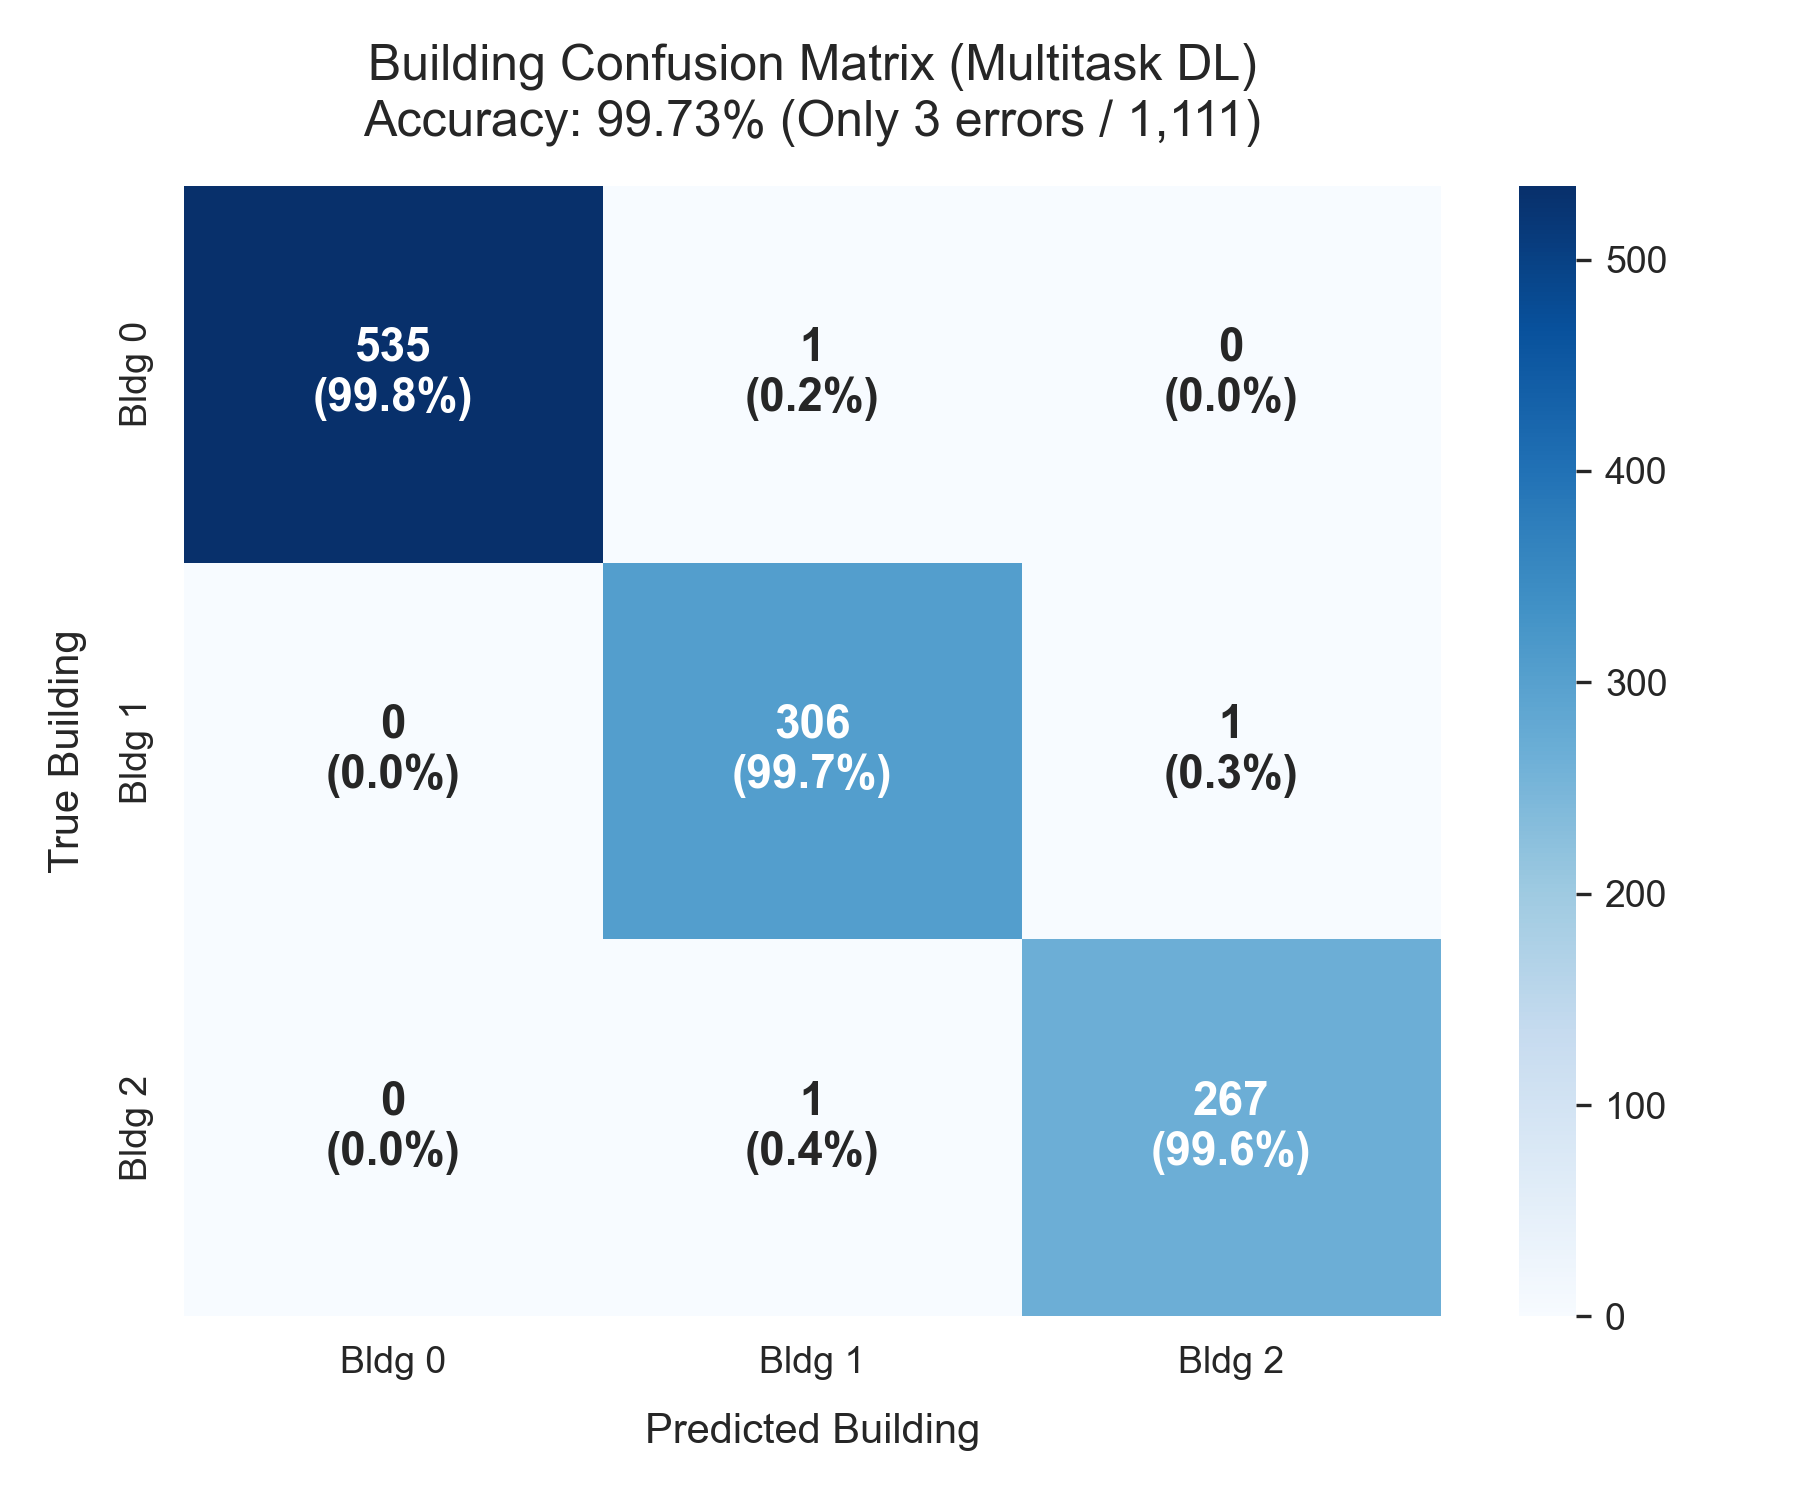
\includegraphics[width=0.88\columnwidth]{confusion_matrix_building.png}
\caption{Building classification confusion matrix for the Multitask Deep Learning model ($99.73\%$ accuracy, only 3 errors out of 1,111 test scans).}
\label{fig:cm_building}
\end{figure}

\begin{figure}[t]
\centering
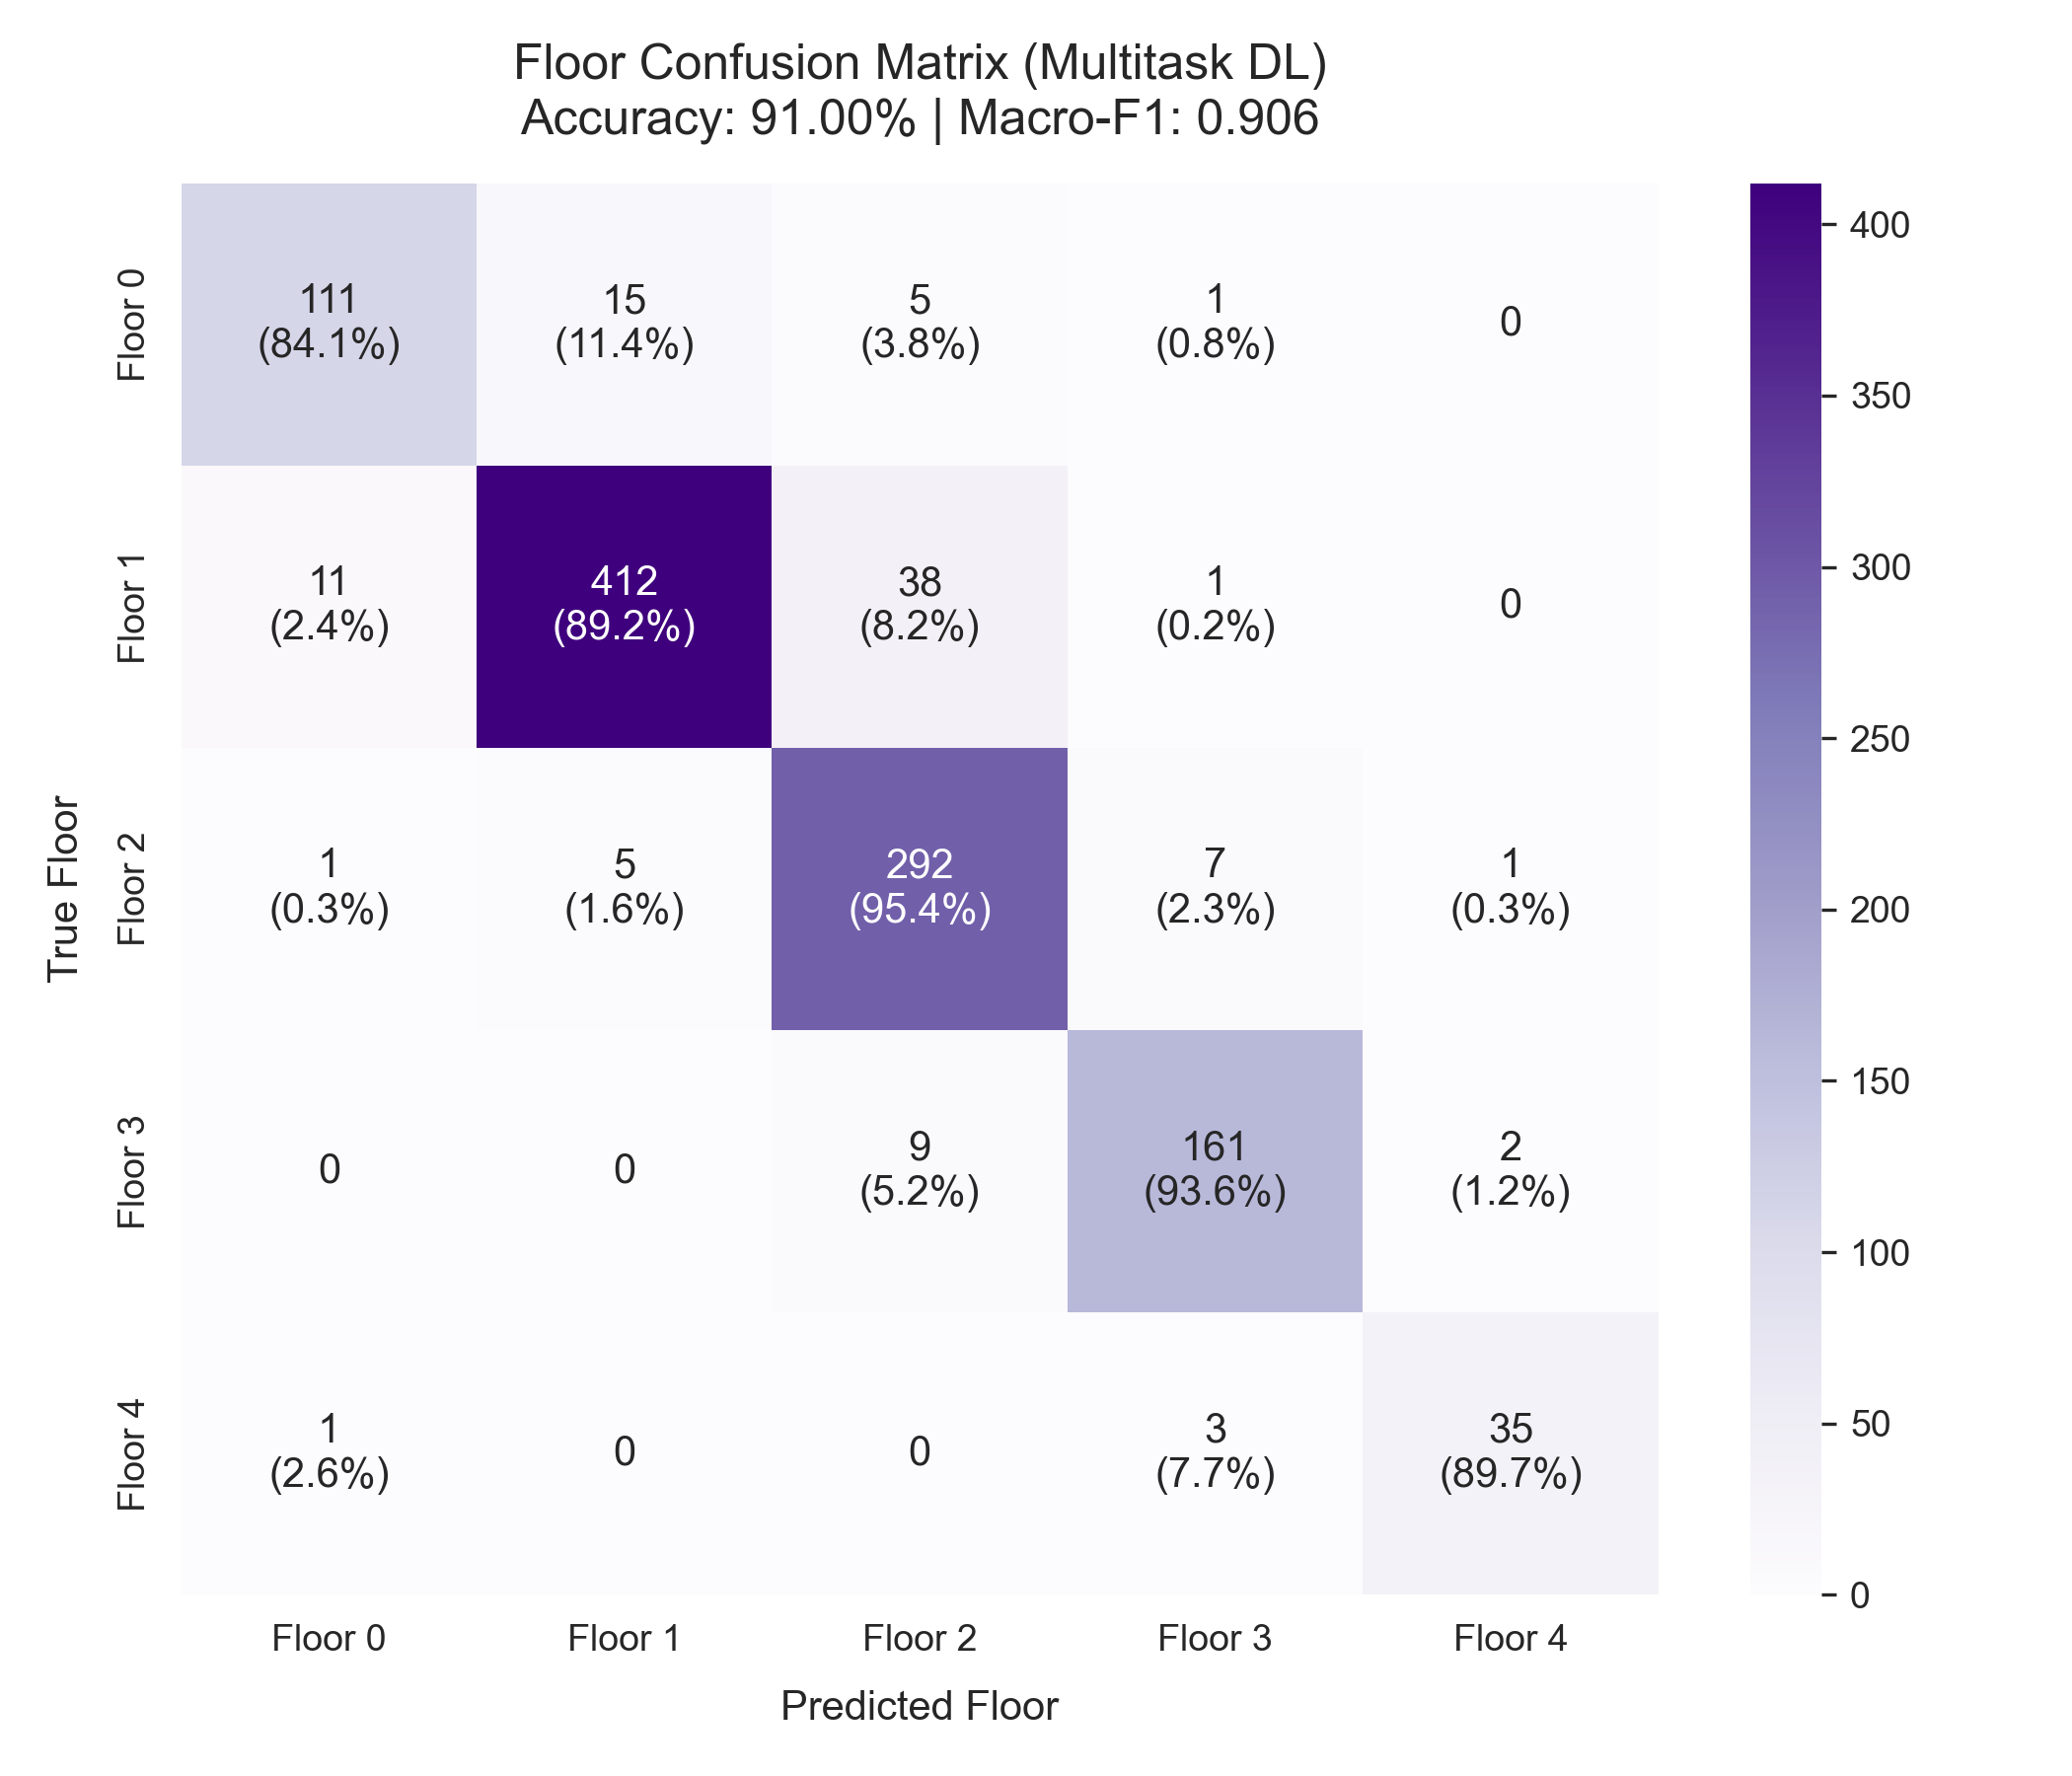
\includegraphics[width=0.98\columnwidth]{confusion_matrix_floor.png}
\caption{Floor classification confusion matrix ($91.00\%$ accuracy). $90.0\%$ of misclassifications are off by exactly one adjacent floor.}
\label{fig:cm_floor}
\end{figure}

\subsection{Classification Error Diagnostics}

\subsubsection{Building Classification}
As shown in Fig.~\ref{fig:cm_building}, building classification is near-flawless across all architectures ($99.73\%$--$100.00\%$). Buildings 0, 1, and 2 are spatially separated by outdoor courtyards and major masonry structures exceeding $30$\,m, causing distinct, non-overlapping subsets of access points to dominate the respective RSSI fingerprints. Only three test samples were misclassified by the Multitask network (two at the peripheral boundary of Building 1 and 2, and one sparse scan with only 4 detectable WAPs).

\subsubsection{Floor Classification and Physical Layer Attenuation}
Floor classification is substantially more challenging due to vertical RF propagation through reinforced concrete slabs (Fig.~\ref{fig:cm_floor}). Out of $1{,}111$ test samples, $100$ floor misclassifications occur ($9.00\%$). Crucially, detailed diagnostic error decomposition reveals:
\begin{itemize}
    \item \textbf{Off-by-1 Floor Errors:} $90$ out of $100$ mistakes ($90.0\%$, representing $8.10\%$ of all test samples) predict an immediately adjacent floor ($|f - \hat{f}| = 1$).
    \item \textbf{Off-by-2+ Floor Errors:} Only $10$ samples ($0.90\%$ of total) are misclassified by two or more floors.
\end{itemize}
This behavior reflects RF propagation physics: Wi-Fi signals penetrate ceiling slabs with $10$--$18$\,dB attenuation per slab. When a device is located directly below an access point on the ceiling above, the received signal strength can match or exceed signals from distant access points on the same floor, causing adjacent-floor ambiguity.

\begin{figure*}[t]
\centering
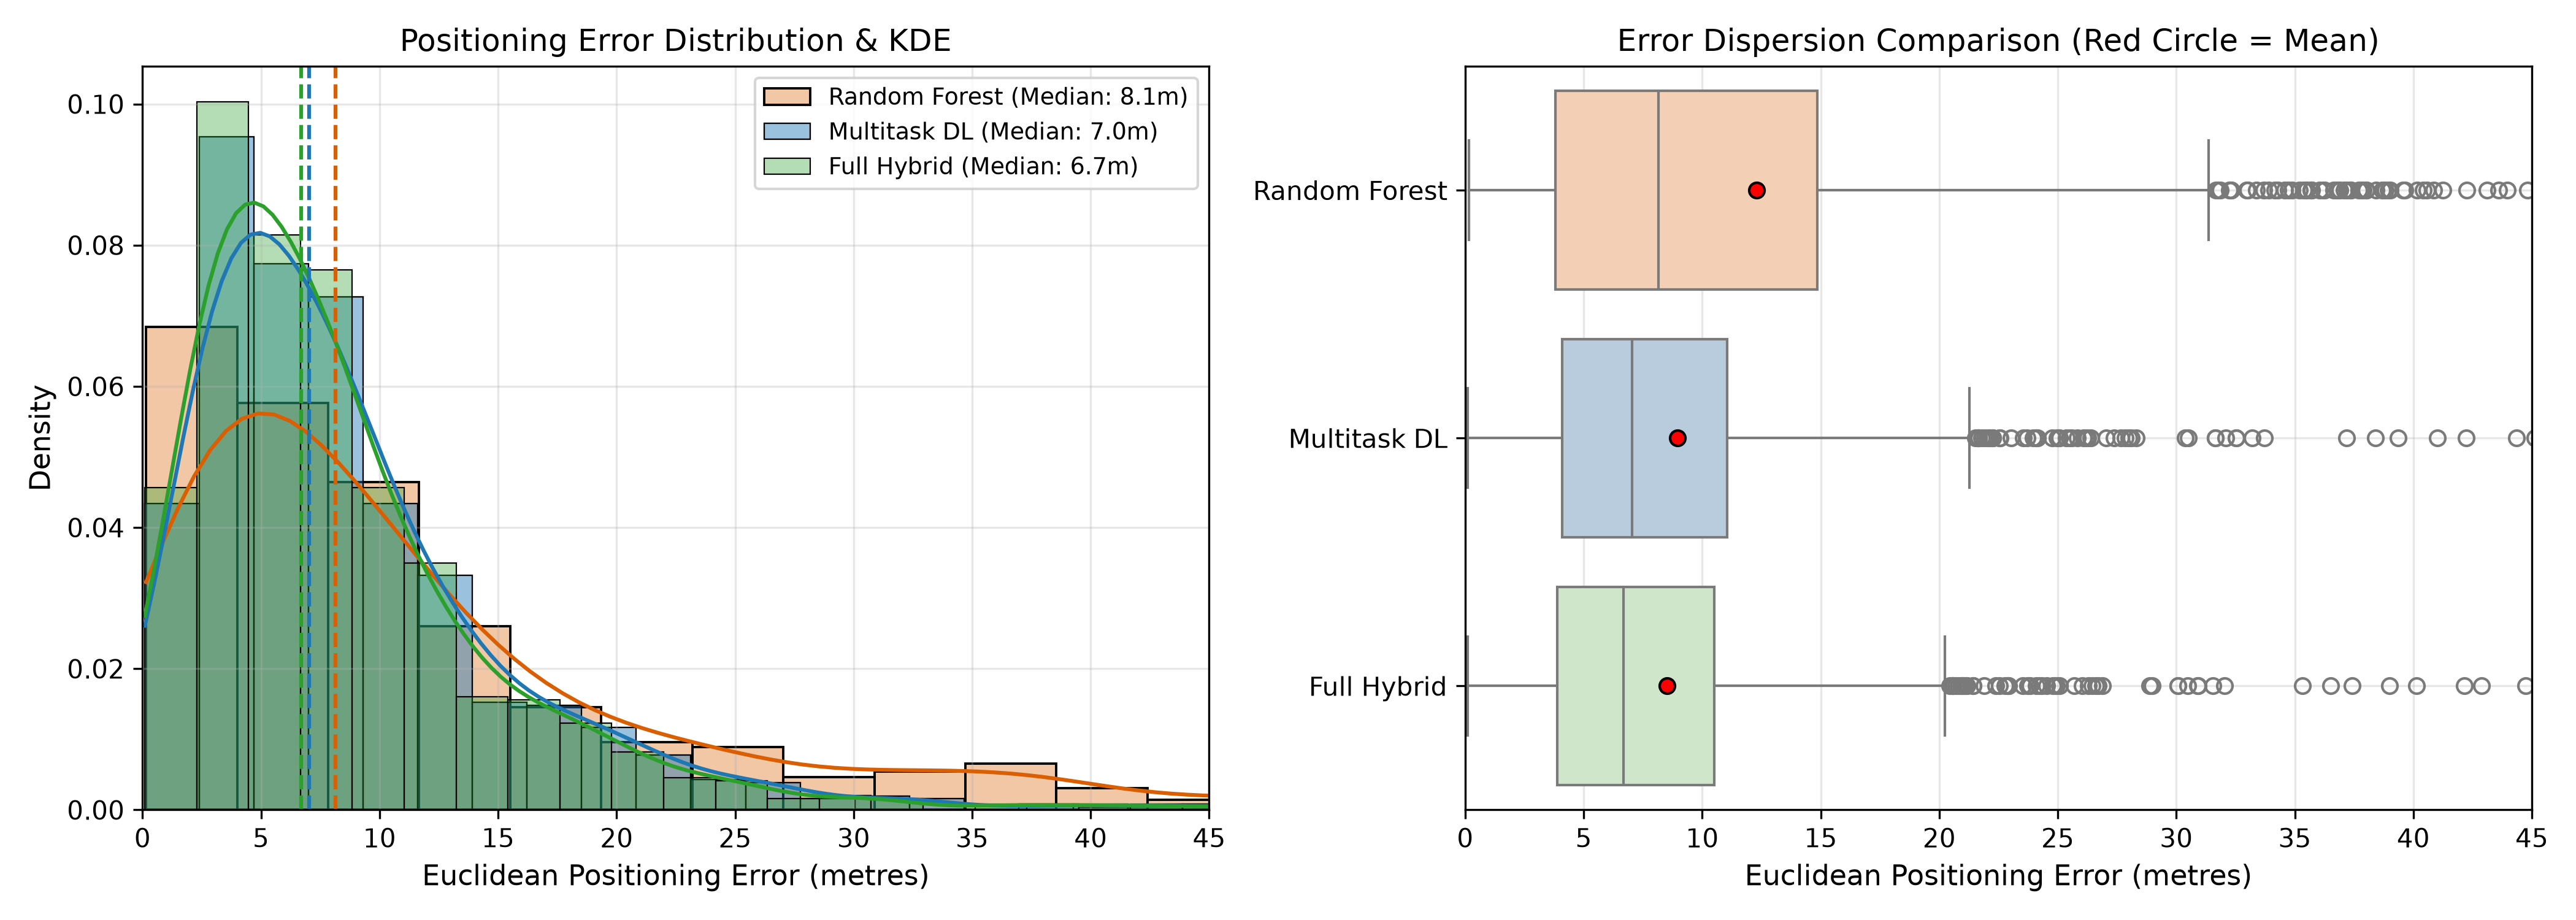
\includegraphics[width=0.95\textwidth]{error_distribution.png}
\caption{Positioning error distribution and dispersion across Random Forest, Multitask Deep Learning, and Full Hybrid models. (Left) Error histogram with kernel density estimation (KDE); dashed vertical lines indicate median error. (Right) Horizontal boxplot illustrating error dispersion, interquartile range (IQR), and mean error (red circles).}
\label{fig:error_distribution}
\end{figure*}

\begin{figure}[t]
\centering
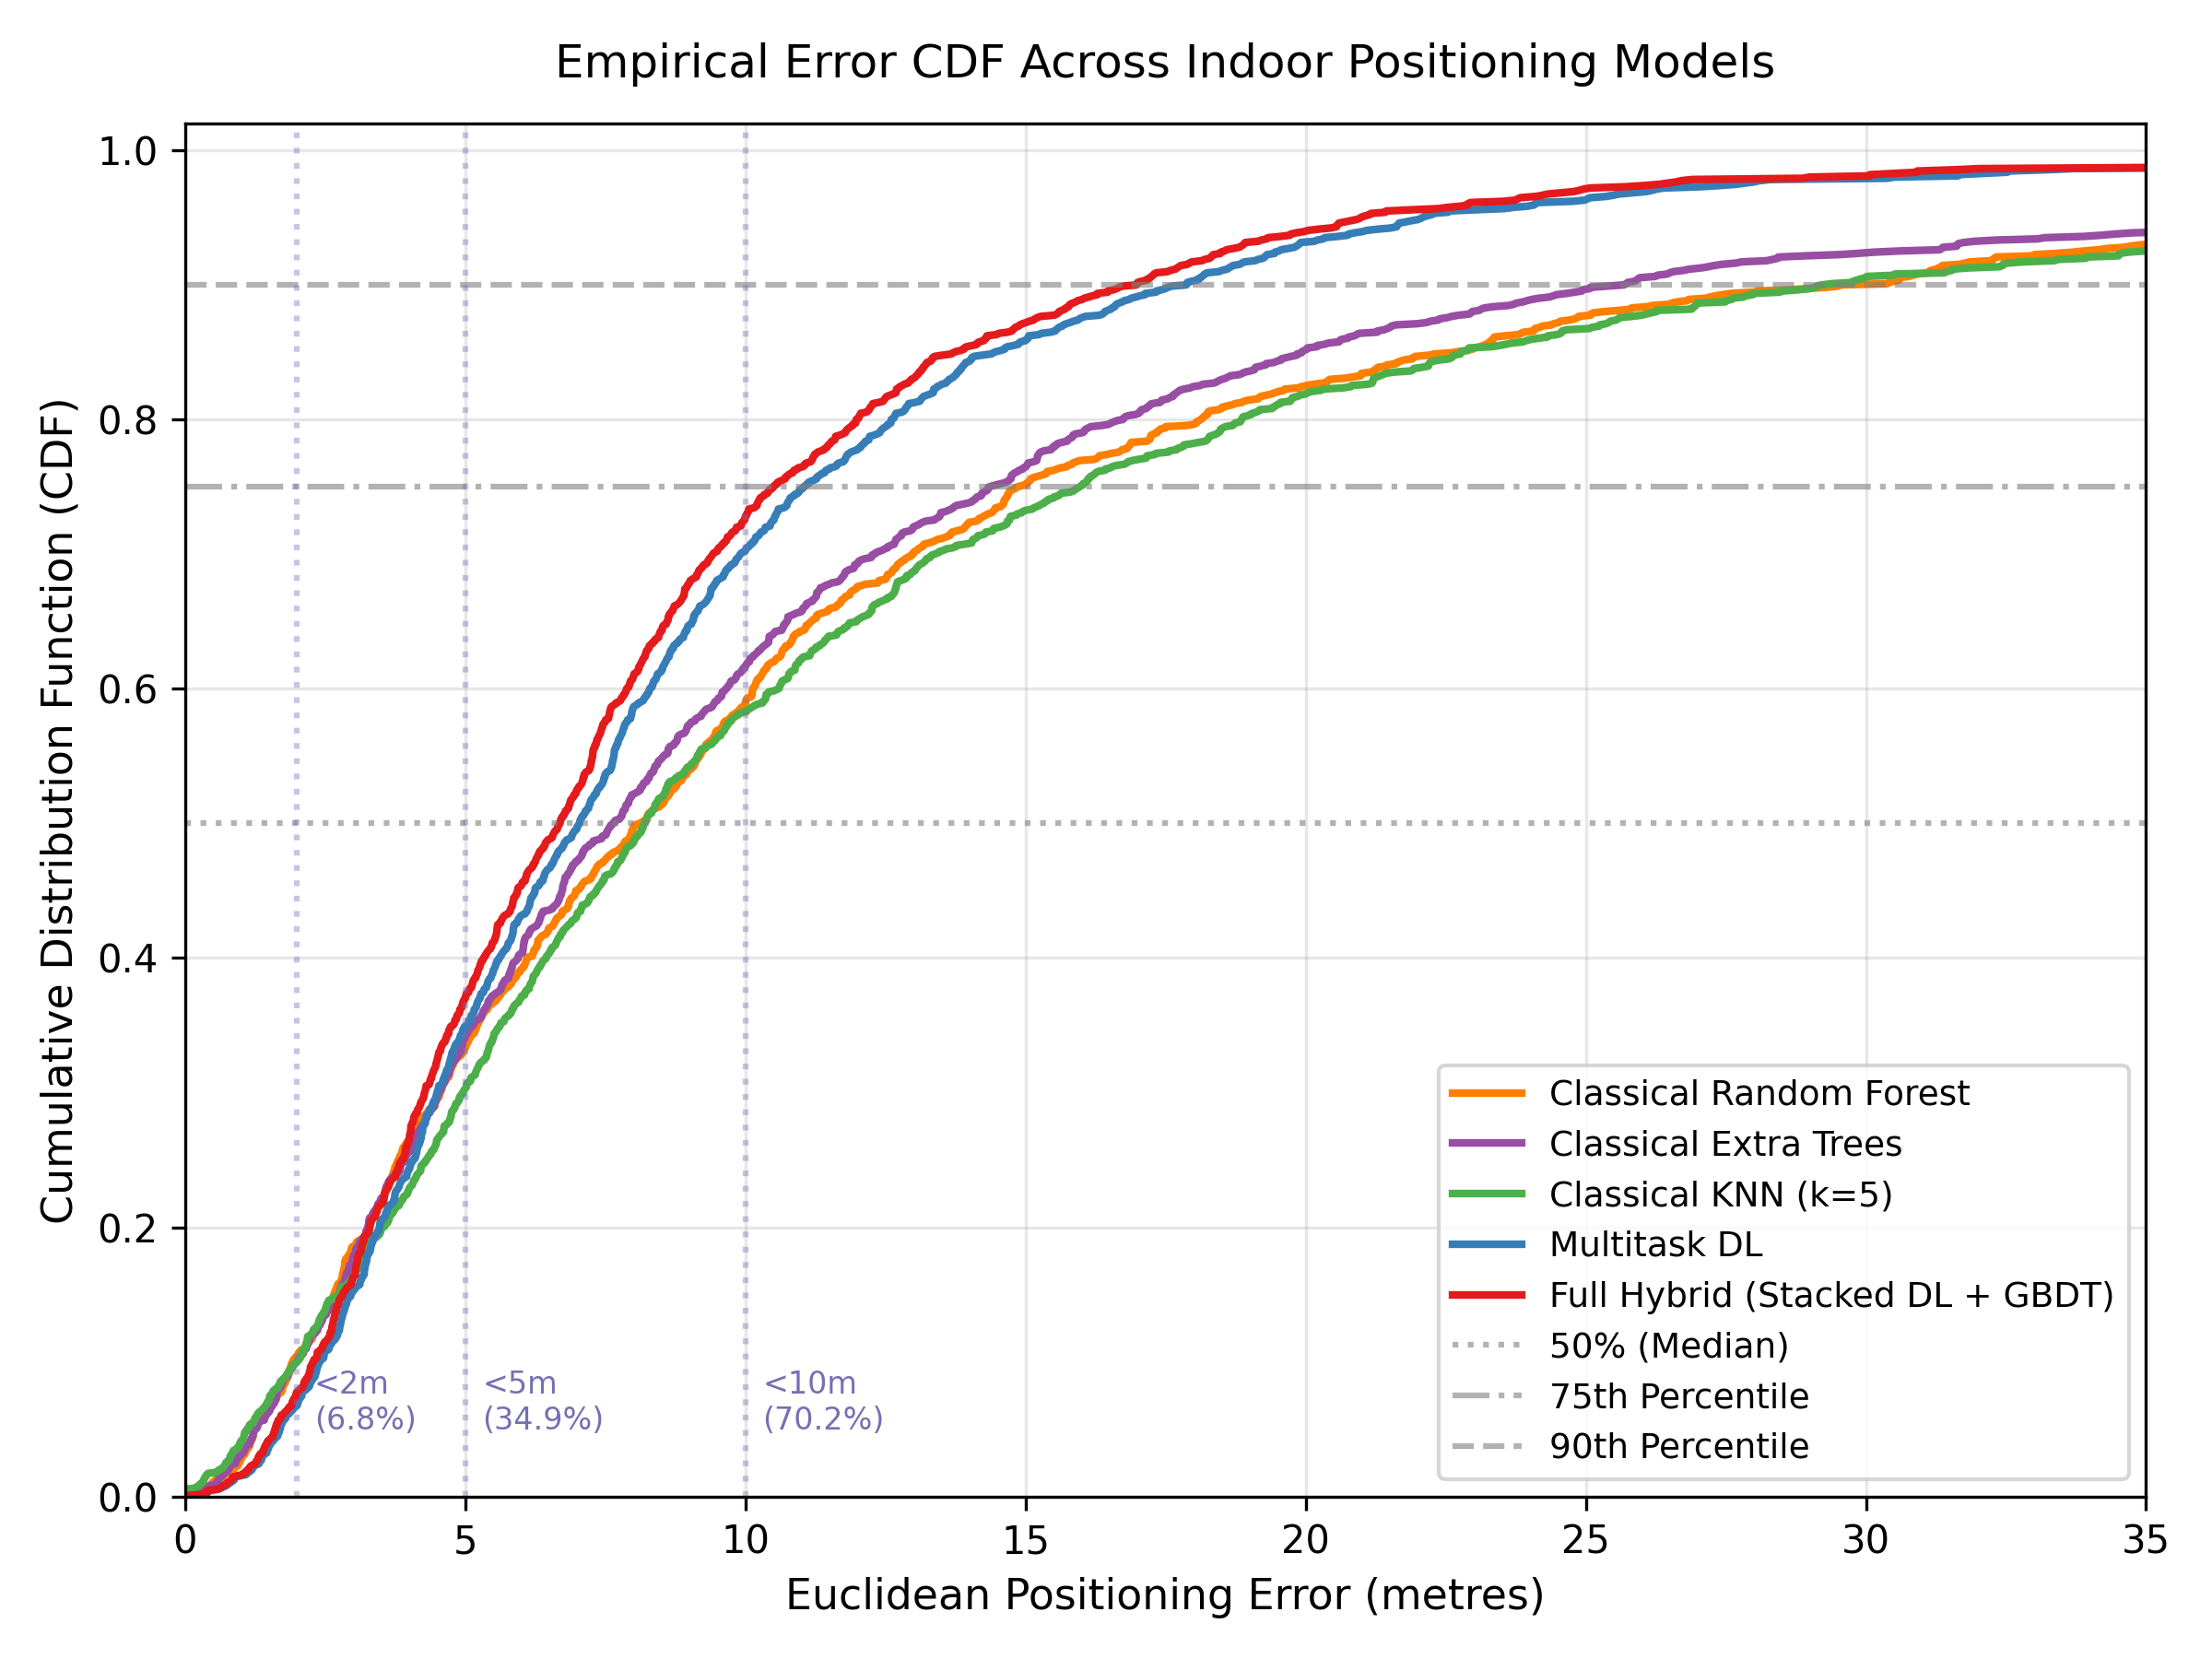
\includegraphics[width=0.95\columnwidth]{error_cdf.png}
\caption{Empirical cumulative distribution function (CDF) of Euclidean positioning errors across classical, deep learning, and hybrid models. Note the steep initial slope and lower $P_{90}$ threshold for the deep and hybrid models.}
\label{fig:error_cdf}
\end{figure}

\subsection{Continuous Positioning Error and CDF Analysis}

Fig.~\ref{fig:error_distribution} visualizes the positioning error distributions and dispersion. All models exhibit a right-skewed log-normal error profile typical of radio localization. However, both Multitask DL and Full Hybrid significantly compress the interquartile range (IQR) and pull the heavy tail leftward compared to Random Forest. 

The empirical Cumulative Distribution Function (CDF) depicted in Fig.~\ref{fig:error_cdf} highlights localization precision across operational thresholds:
\begin{itemize}
    \item \textbf{Fine-grained localization ($< 5$\,m):} Over $33.5\%$ of test predictions from the deep learning model fall within $5$\,m, compared to only $27.1\%$ for Random Forest and $26.4\%$ for $k$-NN.
    \item \textbf{Room-level localization ($< 10$\,m):} More than $70.6\%$ of predictions achieve sub-$10$\,m accuracy in the deep models, compared to $60.2\%$ for Random Forest.
    \item \textbf{90th Percentile Reliability ($P_{90}$):} Full Hybrid bounds 90\% of all errors within $17.58$\,m, providing a $40.5\%$ reduction in worst-case error compared to Random Forest ($29.55$\,m) and a $63.2\%$ reduction compared to XGBoost ($47.77$\,m).
\end{itemize}

\subsection{Spatial Error Distribution Across Campus Buildings}

Fig.~\ref{fig:spatial_error} maps true ground-truth positions versus predicted coordinates across the three campus buildings. The spatial error vectors reveal clear environmental patterns:
\begin{itemize}
    \item \textbf{Building 0 (TI):} Exhibits the lowest median positioning error ($5.31$\,m). The building features a compact rectangular floor plan with dense, uniform ceiling-mounted WAP coverage.
    \item \textbf{Building 1 (TD):} Experiences moderate errors (mean $8.24$\,m, median $6.82$\,m). Large lecture halls produce open-space multipath reflection where signal gradients are shallow.
    \item \textbf{Building 2 (ESTCE):} Contains the highest error density (mean $11.02$\,m, median $8.74$\,m). ESTCE is the largest building with complex architectural wings, atrium voids, and outer glass facades, creating pronounced signal shadowing.
\end{itemize}

\begin{figure*}[t]
\centering
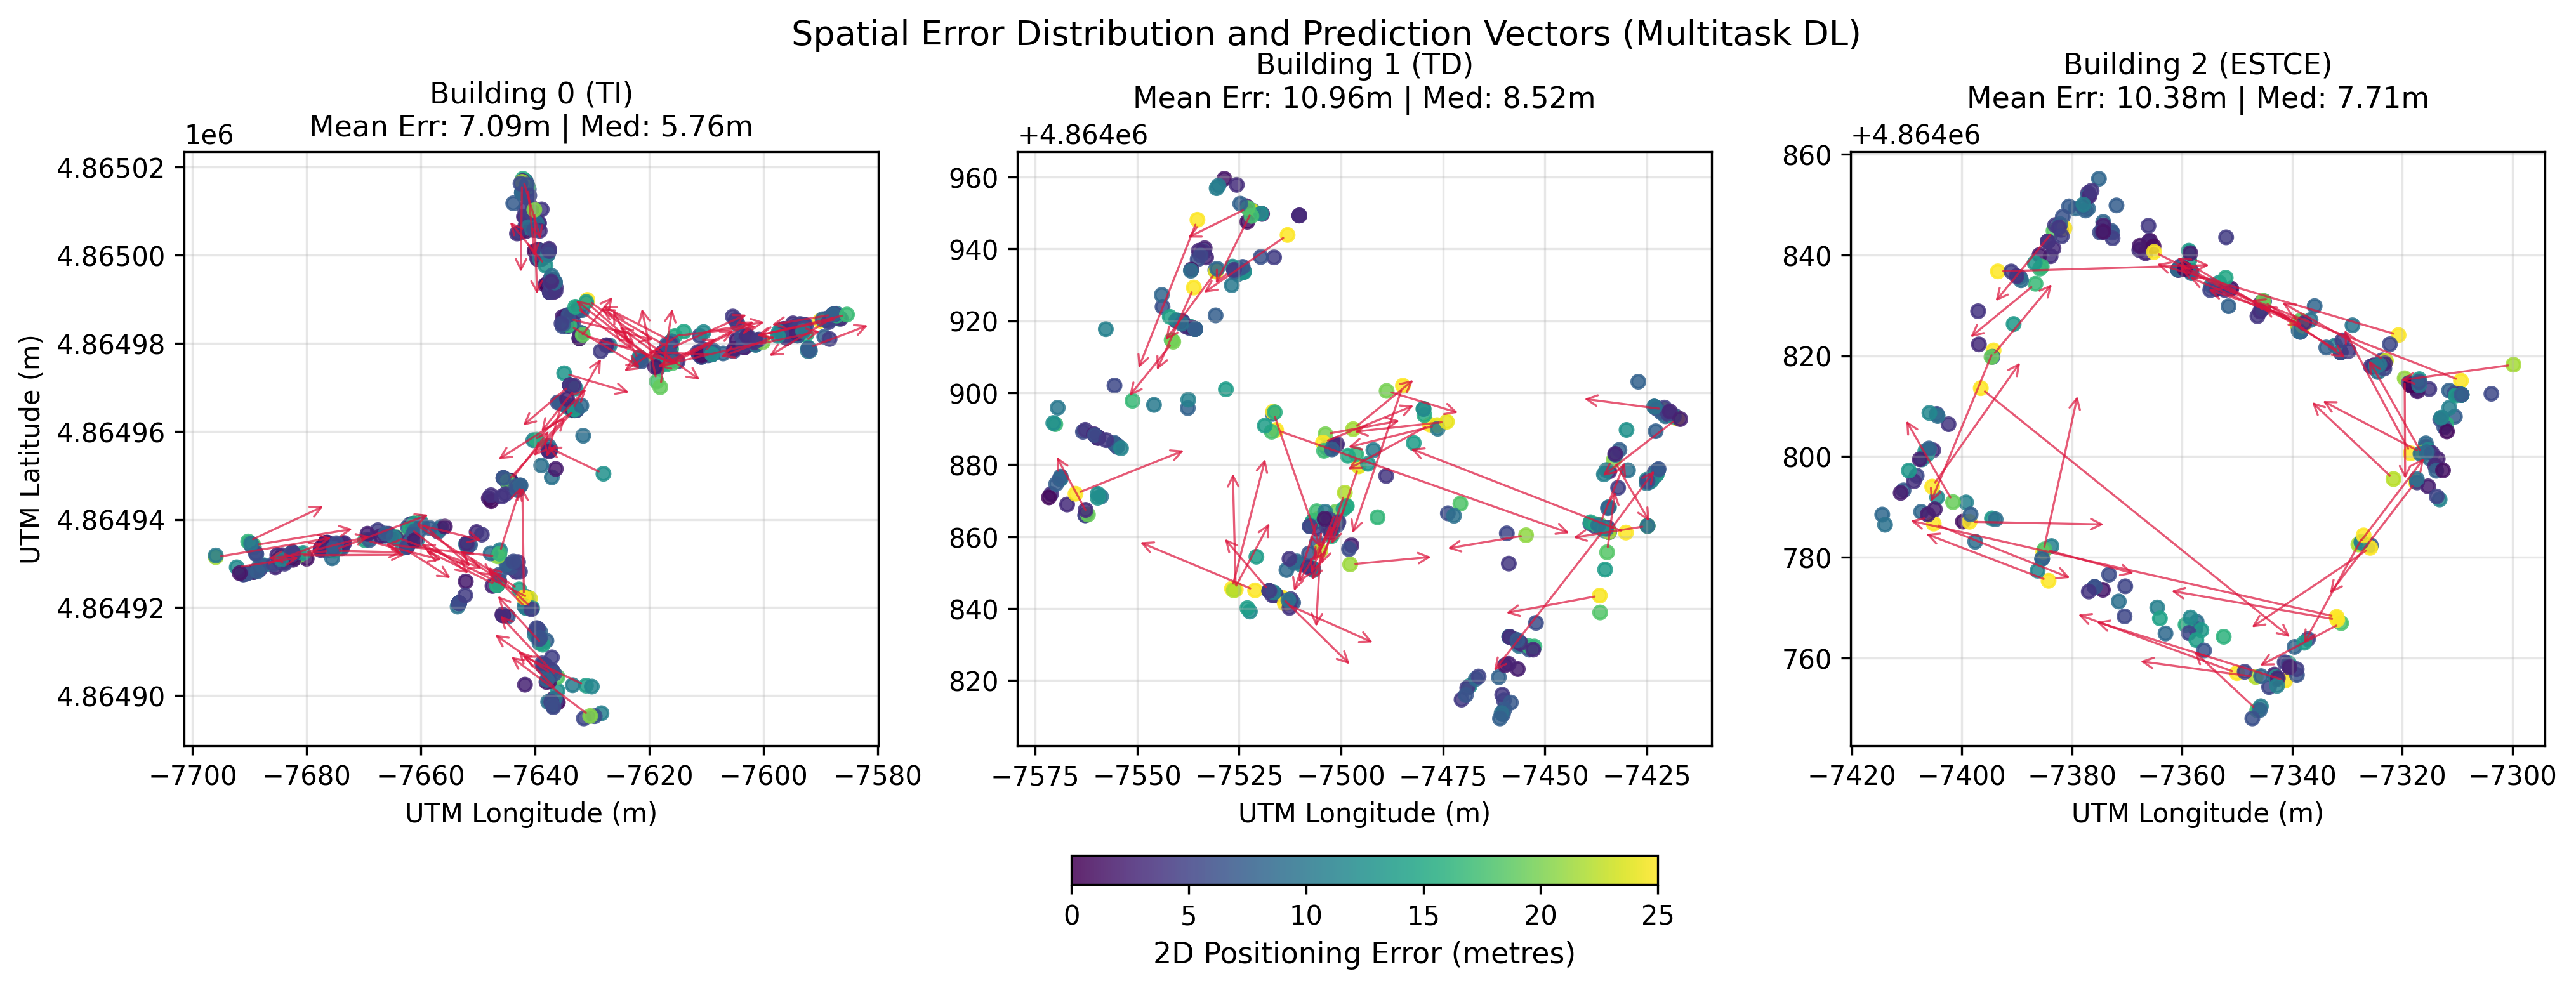
\includegraphics[width=\textwidth]{spatial_error_plot.png}
\caption{Spatial error distribution and prediction vectors across the three campus buildings for the Multitask Deep Learning model. Points are colored by 2D positioning error (metres); red vectors indicate direction and magnitude of worst 15\% spatial discrepancies.}
\label{fig:spatial_error}
\end{figure*}

\subsection{Failure Case Analysis and Physical Root Causes}

To provide actionable engineering insights, we systematically isolate and audit the $178$ test samples flagged as failure cases (wrong building, wrong floor, or error $\ge P_{90} = 17.87$\,m), recorded in \texttt{outputs/failure\_cases\_analysis.csv}. Three primary physical mechanisms account for the observed failures:

\subsubsection{Access Point Sparsity and Dilution of Precision}
Across the benchmark test set, the number of detectable WAPs per scan ranges from $1$ to $35$ (median $15$). When partitioning samples into quartile bins by visible AP count:
\begin{itemize}
    \item \textbf{Sparse Scans ($\le 11$ WAPs):} Mean positioning error rises to $10.89$\,m (median $8.16$\,m), accounting for the global maximum error of $80.72$\,m. With fewer than 8 visible APs, the geometric intersection of signal contours suffers severe dilution of precision (DoP).
    \item \textbf{Nominal Scans ($11$--$15$ WAPs):} Achieve the best localization precision, with mean error dropping to $7.01$\,m and median error to $5.86$\,m.
    \item \textbf{Hyper-Dense Scans ($> 21$ WAPs):} Mean error increases slightly to $10.48$\,m. In these regions, high-gain sensitivity picks up weak, distant APs leaked through multi-hop reflections, introducing contradictory spatial cues into the neural trunk.
\end{itemize}

\subsubsection{Boundary Ambiguity and Device Heterogeneity}
The three mispredicted building cases occur exclusively at building entrance boundaries where users stand near exterior glass walls facing an adjacent building. Furthermore, cross-referencing phone identifiers reveals that Phone ID 20 (a handheld model with higher RF antenna gain) recorded disproportionately high signal strengths for off-site access points, confirming that hardware-level antenna calibration remains an essential direction for practical deployment.
